%!TEX TS-program = xelatex
\documentclass[12pt, a4paper]{article}  

\usepackage{etex} % расширение классического tex в частности позволяет подгружать гораздо больше пакетов, чем мы и займёмся далее

%%%%%%%%%% Математика %%%%%%%%%%
\usepackage{amsmath,amsfonts,amssymb,amsthm,mathtools} 
%\mathtoolsset{showonlyrefs=true}  % Показывать номера только у тех формул, на которые есть \eqref{} в тексте.
%\usepackage{leqno} % Нумерация формул слева


%%%%%%%%%%%%%%%%%%%%%%%% Шрифты %%%%%%%%%%%%%%%%%%%%%%%%%%%%%%%%%
\usepackage{fontspec}         % пакет для подгрузки шрифтов
\setmainfont{Arial}   % задаёт основной шрифт документа

\defaultfontfeatures{Mapping=tex-text}

% why do we need \newfontfamily:
% http://tex.stackexchange.com/questions/91507/
\newfontfamily{\cyrillicfonttt}{Arial}
\newfontfamily{\cyrillicfont}{Arial}
\newfontfamily{\cyrillicfontsf}{Arial}

\usepackage{unicode-math}     % пакет для установки математического шрифта
\setmathfont{Asana-Math.otf}      % шрифт для математики

\usepackage{polyglossia}      % Пакет, который позволяет подгружать русские буквы
\setdefaultlanguage{russian}  % Основной язык документа
\setotherlanguage{english}    % Второстепенный язык документа


%%%%%%%%%% Работа с картинками %%%%%%%%%
\usepackage{graphicx}                  % Для вставки рисунков
\usepackage{graphics} 
\graphicspath{{Pictures/}}    % можно указать папки с картинками
\usepackage{wrapfig}                   % Обтекание рисунков и таблиц текстом
\usepackage{subfigure}                 % для создания нескольких рисунков внутри одного


\begin{document}
\section*{Задание 1.}
\begin{figure}[h!]
\begin{minipage}[h!]{0.32\linewidth}
\center\rotatebox{180}{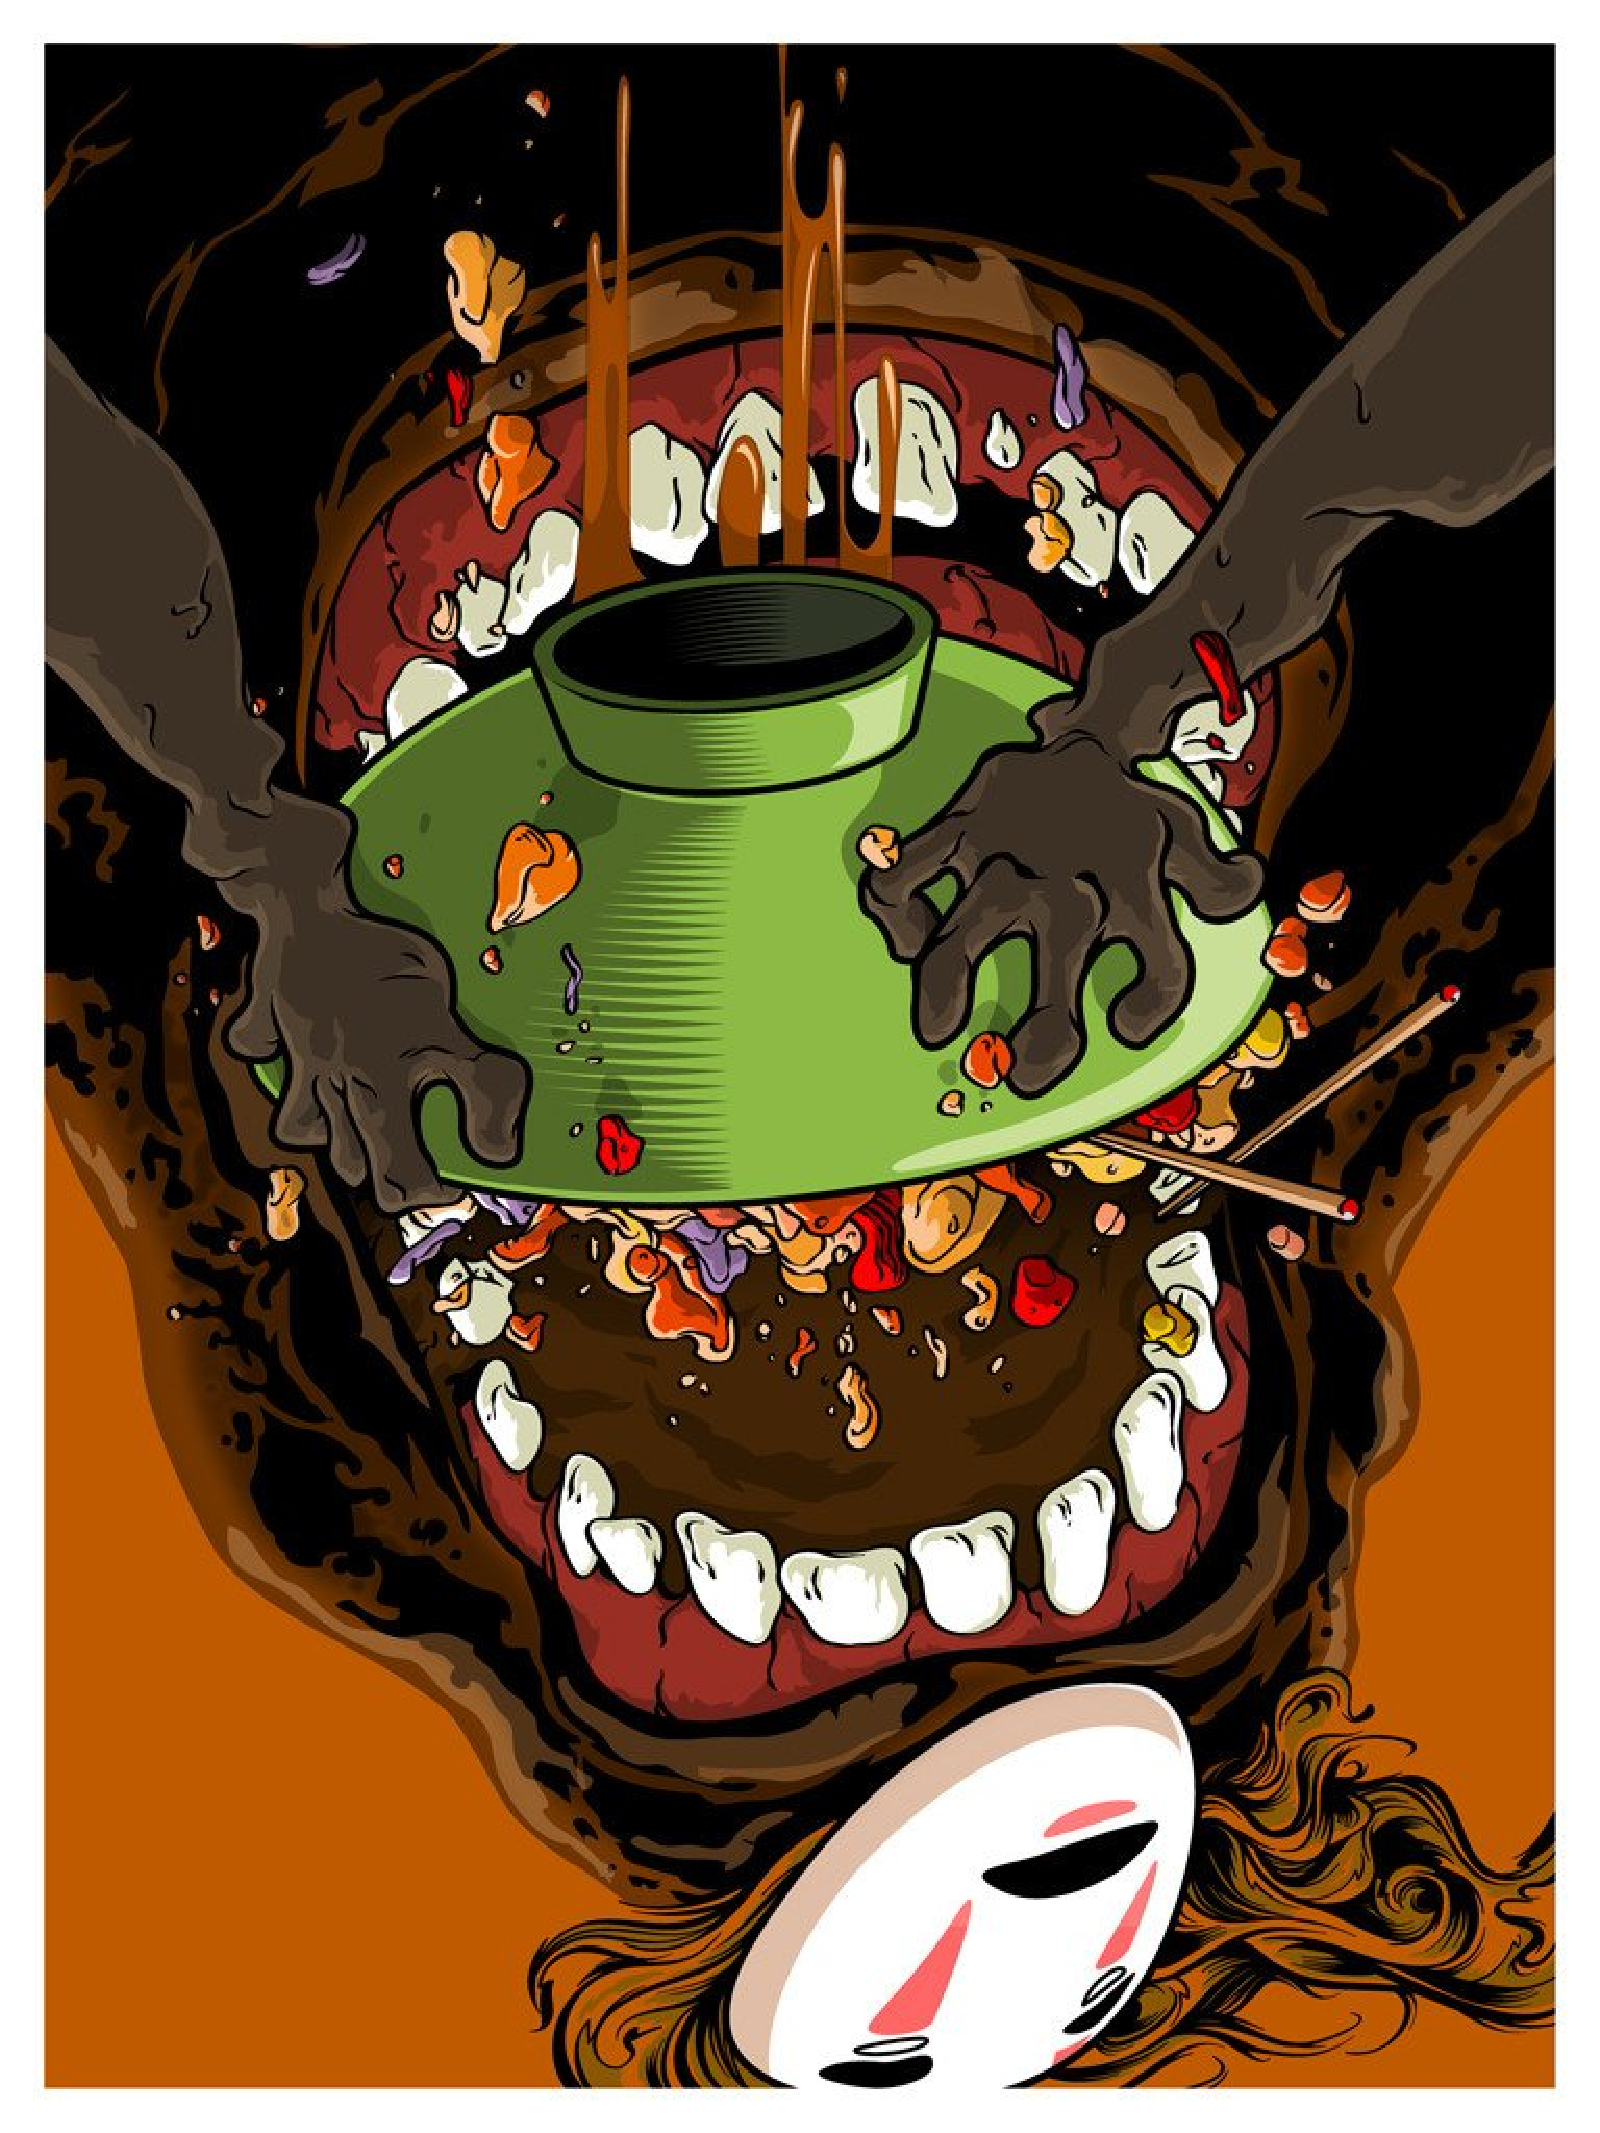
\includegraphics[width=0.8\linewidth]{pop6.pdf}}
\end{minipage}
\hfill
\begin{minipage}[h!]{0.32\linewidth}
\center\includegraphics[width=0.8\linewidth]{pop5.pdf}
\end{minipage}
\hfill
\begin{minipage}[h!]{0.32\linewidth}
\center\rotatebox{180}{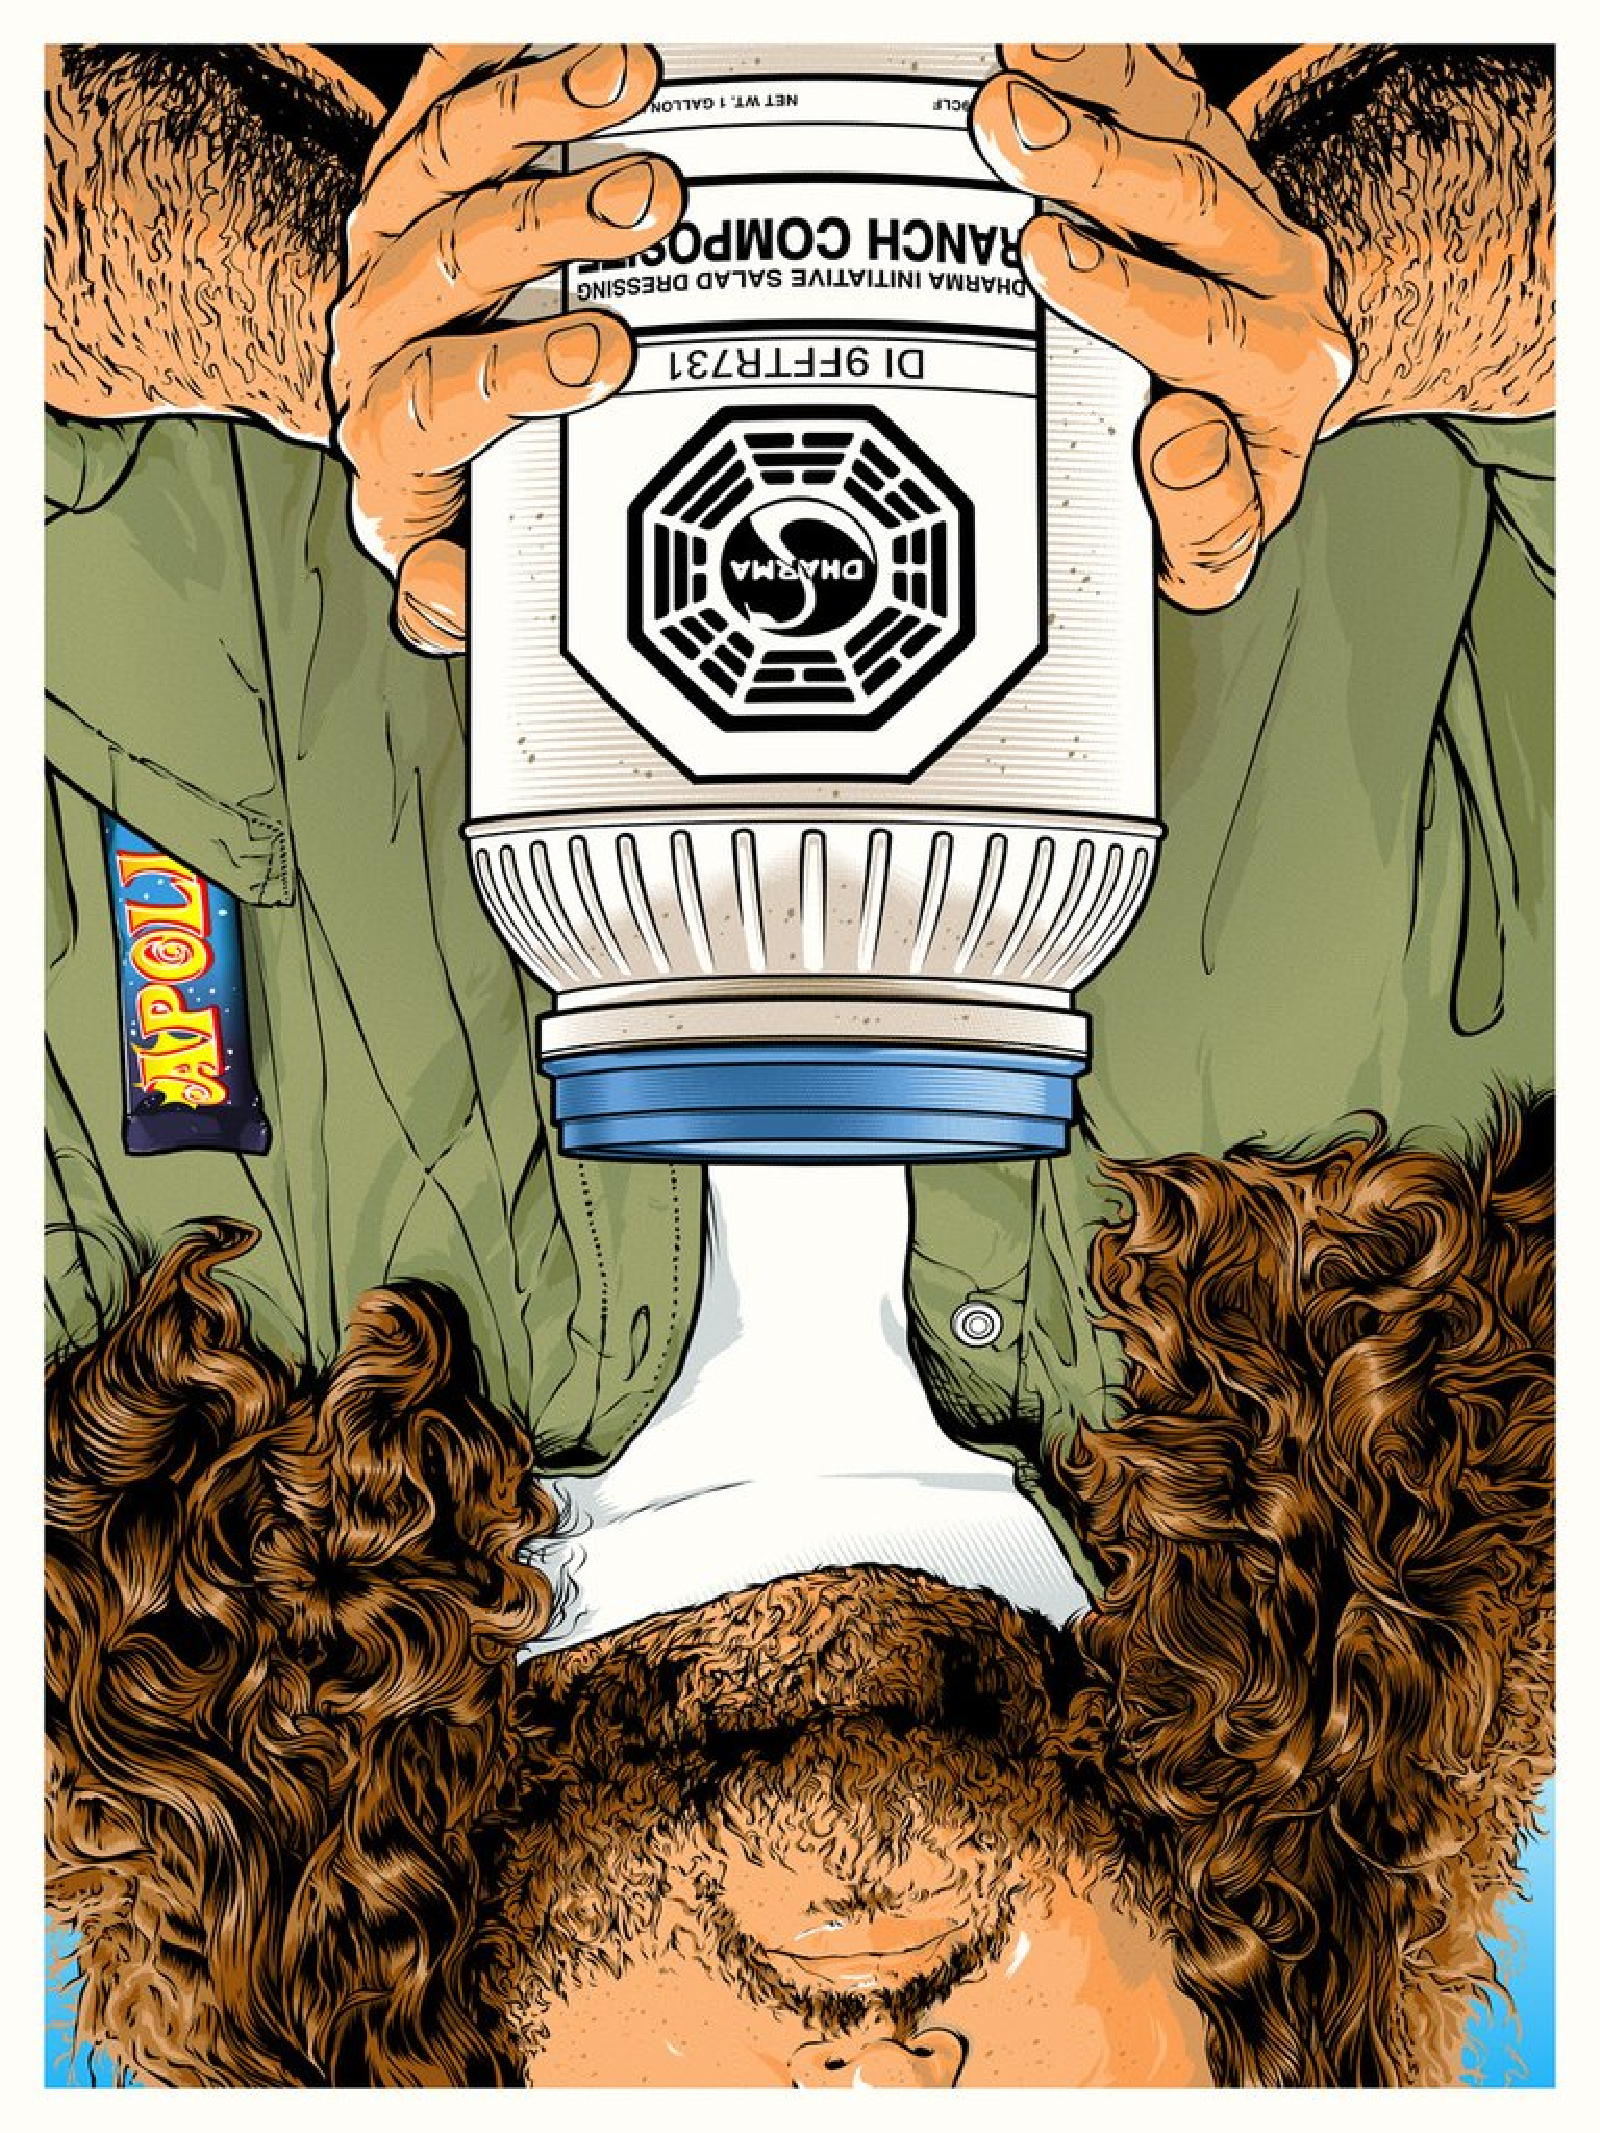
\includegraphics[width=0.8\linewidth]{pop10.pdf}}
\end{minipage}
\vfill
\begin{minipage}[h!]{0.32\linewidth}
\center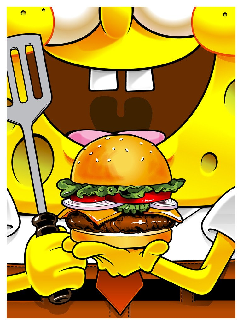
\includegraphics[width=0.78\linewidth]{pop8.pdf}
\end{minipage}
\hfill
\begin{minipage}[h!]{0.34\linewidth}
\center
\includegraphics[width=0.75\linewidth]{pop3.pdf}
\end{minipage}
\hfill
\begin{minipage}[h!]{0.32\linewidth}
\center\rotatebox{270}{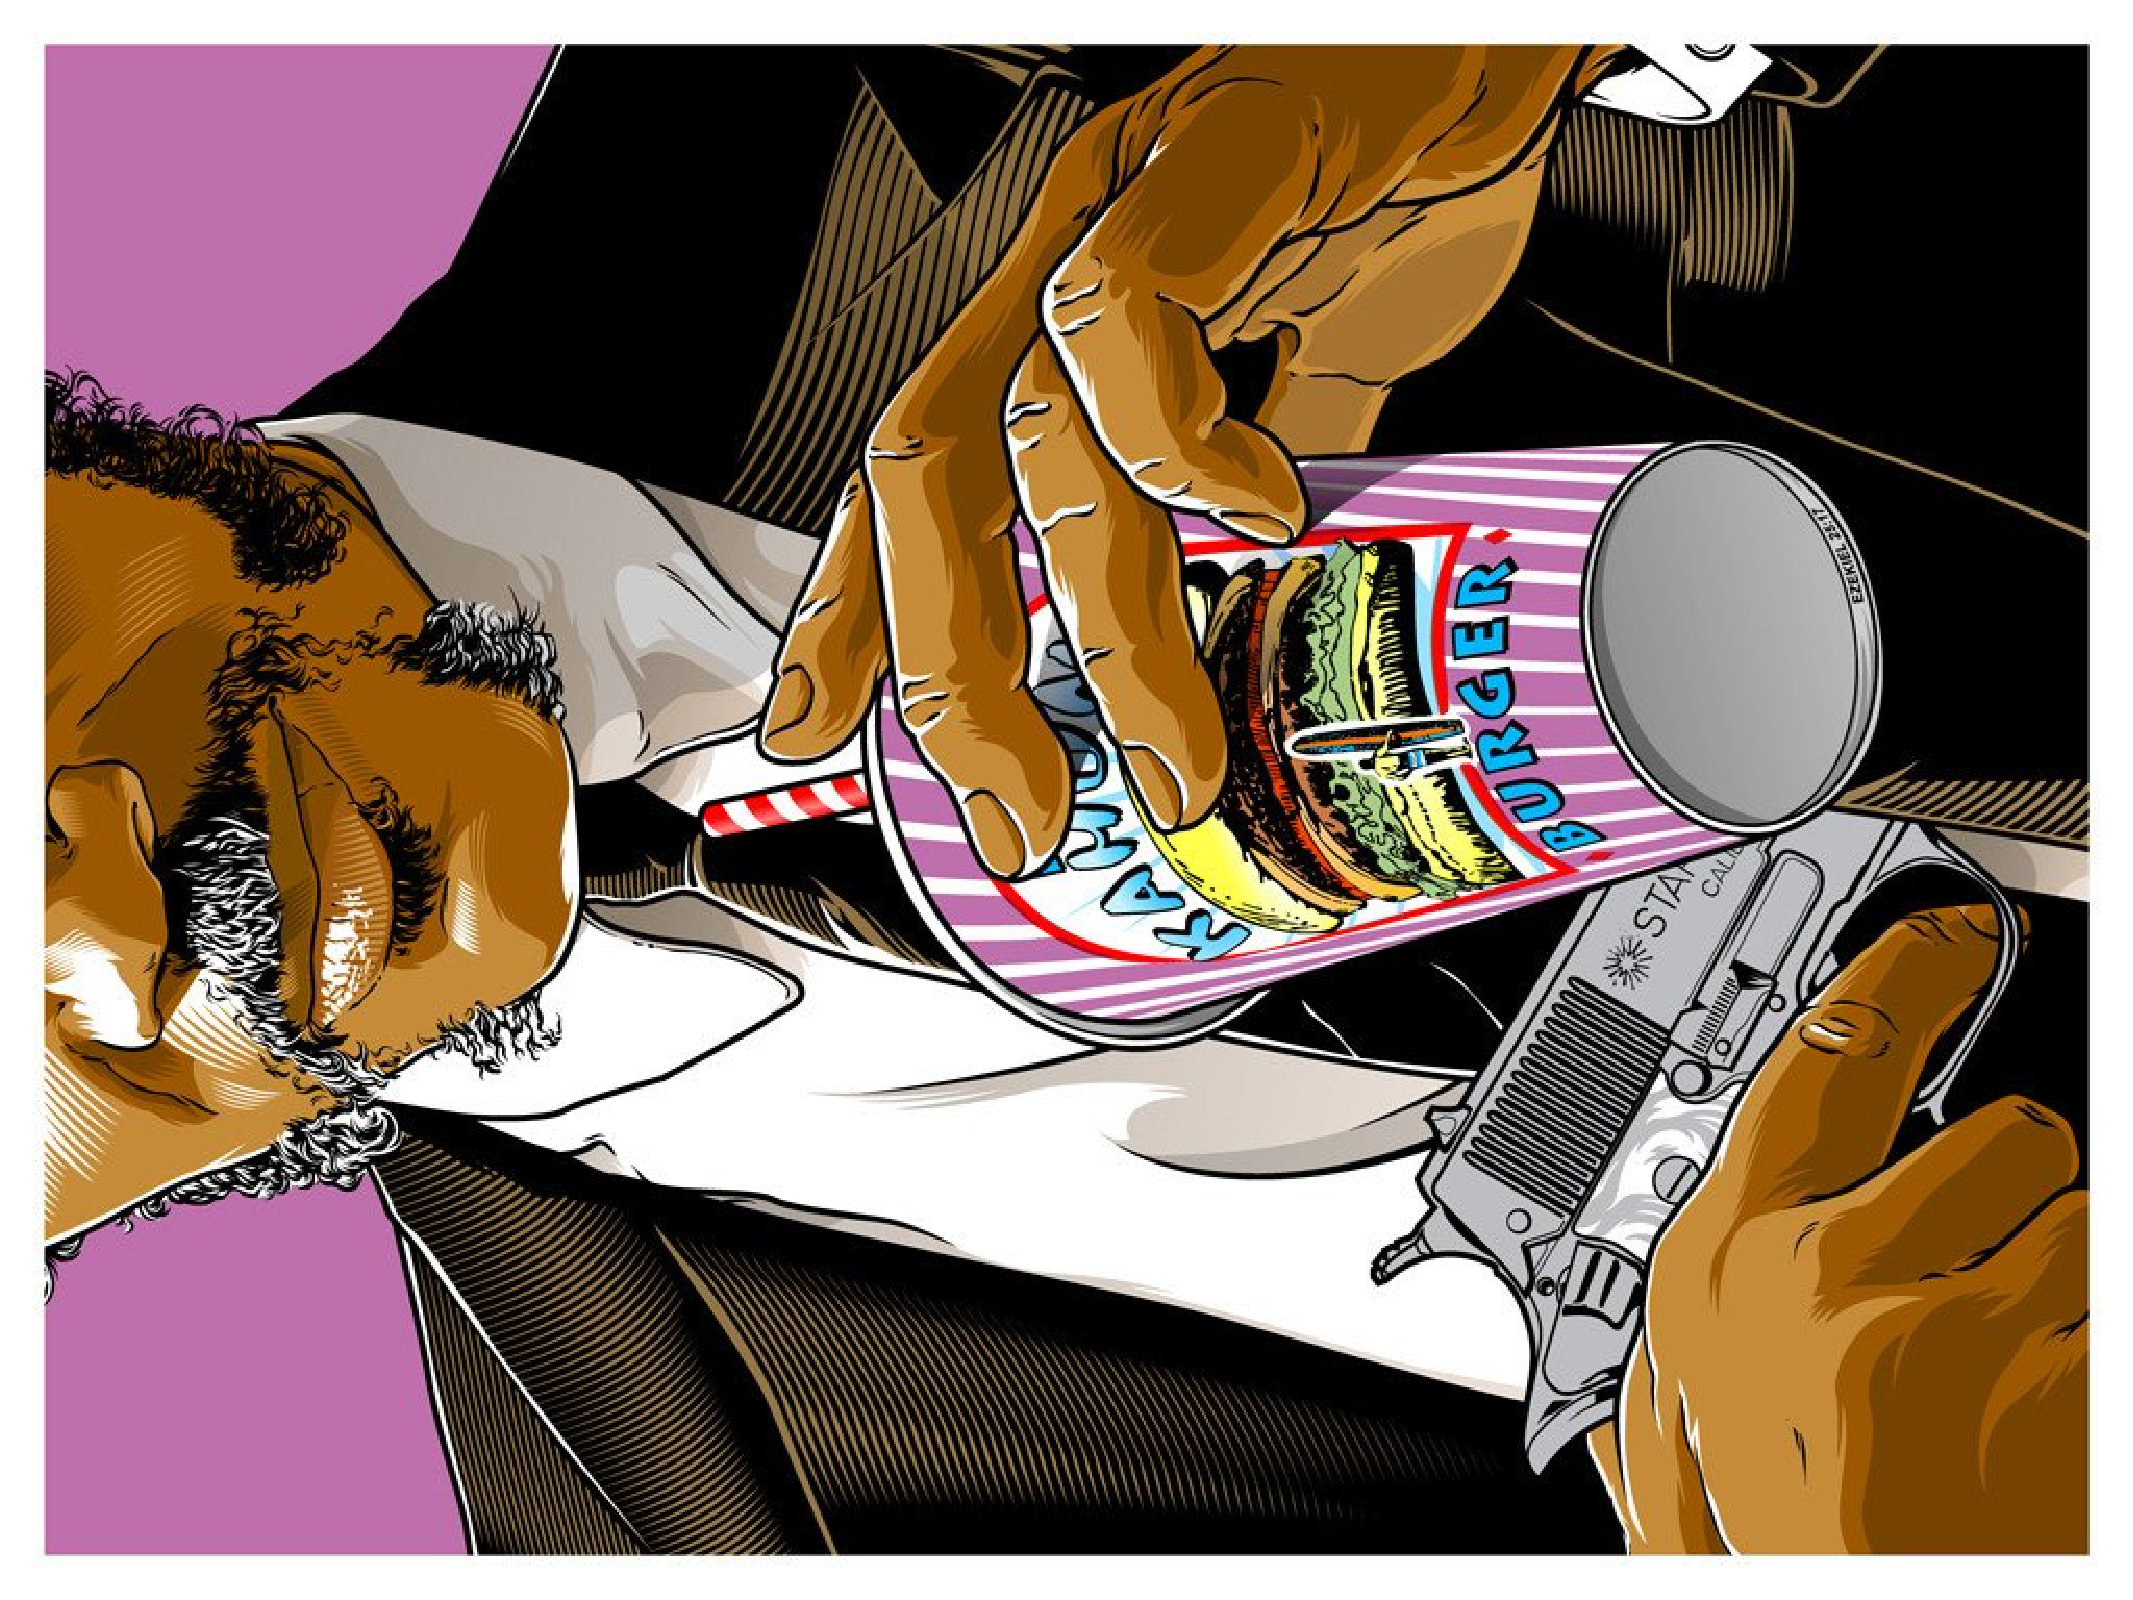
\includegraphics[width=1.065\linewidth]{pop1.pdf}}
\end{minipage}
\caption{Поп-арт}\label{fig:1figs}
\end{figure}
\newpage
\section*{Задание 3.}
\Large{\fontspec{Phorssa}{Уважаемый Филипп! Тебе нужно незамедлительно провести отбор пятерых самых умных студентов отделения экономики и привести их в~назначенное время и в~назначенное место для~ последующего изъятия мозгов. Если требование не~будет выполнено, мы заберем твои мозги. Возможен торг: один умный студент может быть заменен на~двух студентов среднего ума.  \\ 
\begin{flushright}
Пришельцы.
\end{flushright}}}
\end{document}